\begin{landscape}
	\begin{figure}[H]
		\centering
		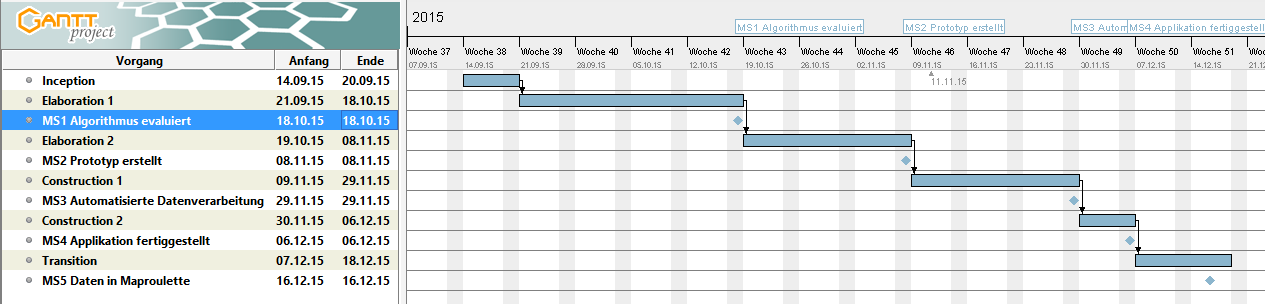
\includegraphics[width=250mm]{images/Gantt.png}
		\caption{Gantt Chart}
	\end{figure}
\section{Risiken}
Um den Problemen, die während des Projekts auftreten können entgegenzuwirken, haben wir eine Risiko Analyse durchgeführt. Diese konnte dann bei der Planung eingesetzt werden.

\subsection{Technische Risiken}
\begin{table}[H]
    \begin{tabular}{|p{0.4cm}|p{1.8cm}|p{7cm}|p{1.5cm}|p{2.25cm}|p{1.75cm}|p{3cm}|p{4cm}|}
    \hline    
    \rowcolor{lightblue}
    Nr & Titel & Beschreibung & maximaler Schaden & Eintrittswahr-scheinlichkeit & Gewichteter Schaden & Vorbeugung & Verhalten beim Eintreten \\ \hline
	R1 & Einarbeitung Python & Python ist den Teammitgliedern teils bekannt, jedoch wurde noch kein grösseres Projekt mit dieser Sprache entwickelt. & 40h & 10\% &4h & Evaluation des Wissensstandes & Informationen bei Studenten einholen, die Python gut kennen \\ \hline
	R2 & Installation OpenCV & Die Installation von OpenCV mit den Contrib Package ist bekanntermassen ein grosse Hürde & 16h & 50\% & 8h & Installation mit Tutorials durchführen & Rücksprache mit Felix Morgner \\ \hline
	R3 & Detektion & Der Algorithmus, der Fussgängerstreifen erkennt, liefert zu schlechte Resultate und kann nicht gebraucht werden. & 40h & 50\% & 20h & Analyse diverser Algorithmen in der Evaluation & Gespräch mit Guido Schuster suchen \\ \hline
	R4 & Download Orthofoto & Download der Orthofotos von Bing oder ähnlichen Quellen ist nicht möglich & 50h & 30\% & 15h & Alternativen im Auge behalten & Auf Bildmaterial der HSR zurückgreifen \\ \hline
	R5 & Software ist zu langsam & Der Download der Orthofotos oder die Detektion kann einige Zeit in Anspruch nehmen.	& 60h & 70\% & 42h & Konzept für Parallelisierung erarbeiten & Fläche einschränken, - Grössere und mehrere Maschinen verwenden. \\ \hline
    \end{tabular}
    \caption[Risiken]{Risiken - Die technischen Risiken wurden zu Beginn des Projektes, wie in der Tabelle ersichtlich, definiert.}
\end{table}
\end{landscape}

\subsection{Auswertung}
\paragraph{R1	Einarbeitung Python}
Risiko ist nicht eingetreten, die Entwickler hatte keine Mühe mit Python zu arbeiten.

\paragraph{R2 Installation OpenCV}
Risiko ist in vollem Umfang eingetreten. Die Installation und Kompilation stellte sich als äusserst Trickreich heraus.

\paragraph{R3 Detektion}
Die Detektion stellte die Hauptaufgabe unserer Arbeit dar, ist jedoch gleichzeitig eine der Risiko reichsten, da Bilderkennung ein nicht ganz triviales Problem ist. Das Implementieren und Testen der verschieden Algorithmen war sehr zeitaufwändig, was dazu führte, dass auch dieses Risiko eingetroffen ist.

\paragraph{R4 Download Orthofoto}
Während des Projektes, wechselten wir mehrmals die API für den Download, was sich auch hier auf einen erhöhten Aufwand auswirkte. 

\paragraph{R5 Software ist zu langsam}
Durch den Einsatz von RQ in Kombination mit Redis wurde diesem Risiko Einhalt geboten. \\

\begin{table}[H]
	\centering
    \begin{tabular}{|p{2cm}|p{5cm}|p{2cm}|}
    \hline    
    \rowcolor{lightblue}
	Nr & Titel & Schaden \\ \hline   
	R1 & Einarbeitung Python & 0h \\ \hline
	R2 & Installation OpenCV & 20h \\ \hline
	R3 & Detektion & 60h \\ \hline
	R4 & Download Orthofoto & 12h \\ \hline
	R5 & Software ist zu langsam & 0h \\ \hline
	\rowcolor{lightblue}
	Total &  & 92h \\ \hline
    \end{tabular}
    \caption[Risikoauswertung]{Risikoauswertung}
\end{table}